\section[Introducción]{Introducción}
\subsection{Contexto}
\begin{frame}
  \frametitle{Contexto}
    \begin{itemize}
      \item La \textbf{metrología monocular} consiste en realizar \textbf{estimaciones de medidas} de la escena a partir de \textbf{una sola vista}.
    \end{itemize}
    \begin{figure}[!ht]
    \begin{center}
        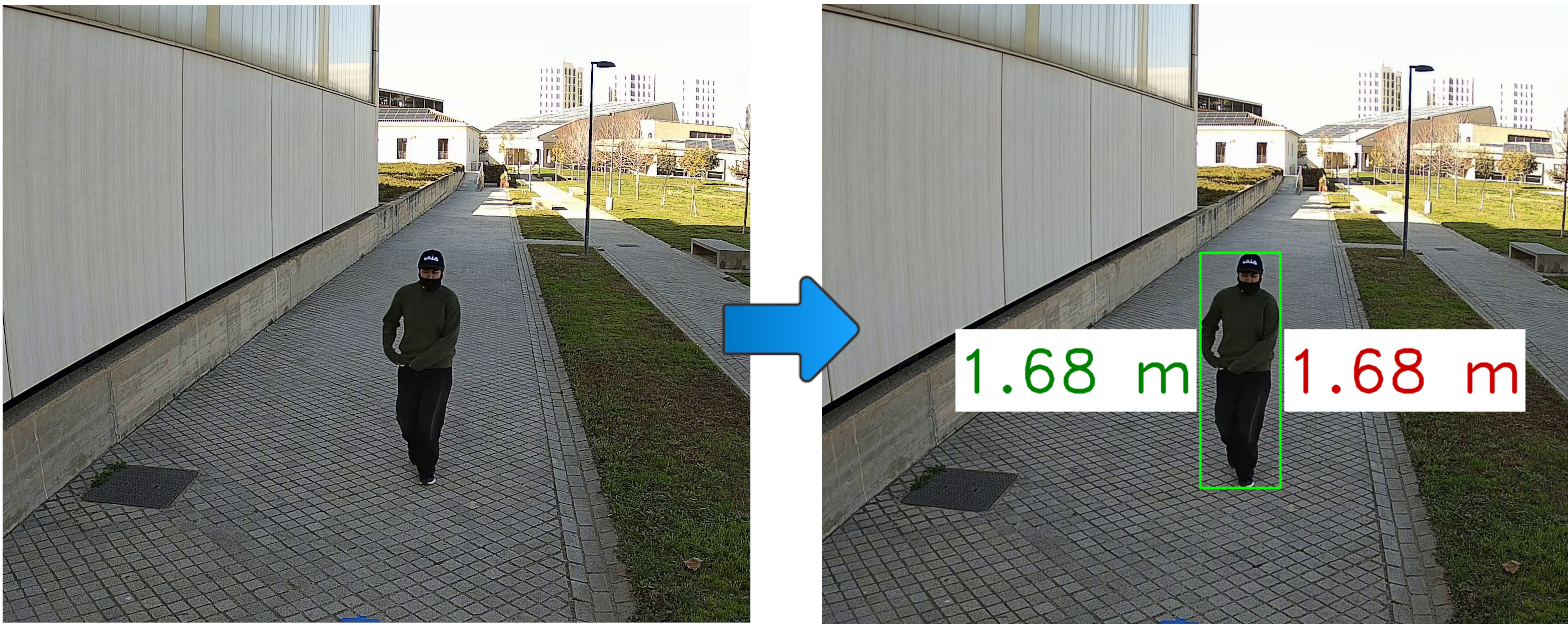
\includegraphics[width=.8\textwidth]{imagenes/chapter1/gimp-tfm-chapter1.png}
    \end{center}
    \caption{Ejemplo de metrología monocular para estimación de altura.}
    \end{figure}
\end{frame}

\note{
Para ilustrar visualmente lo que se busca conseguir con este proyecto, se tiene la siguiente figura
sobre el procedimiento de metrología monocular.
La idea principal es dada una imagen de entrada -- una sola vista de la escena -- poder realizar una
medición en escala absoluta -- es decir, en metros -- de los objetos en escena. Esto abre
puertas a varias aplicaciones que se discutirán a continuación.
}

\begin{frame}
  \frametitle{Motivación}
  \begin{columns}
    \column{0.5\textwidth}
    \begin{itemize}
      \item \textbf{Los métodos clásicos dependen de la calibración} y conocimientos \emph{a priori} de la escena\footnotemark.
      \item El \textbf{auge del aprendizaje profundo} ha abierto nuevas oportunidades.
        \begin{itemize}
          \item \textbf{Desafíos importantes}: ambigüedad inherente a la escala absoluta.
          \item \textbf{Motivación}: La metrología monocular asequible afectaría a múltiples ámbitos industriales y científicos.
        \end{itemize}
    \end{itemize}
    \column{0.5\textwidth}
    \vspace{-.8cm}
    \begin{figure}[!ht]
    \begin{center}
        %\subfloat{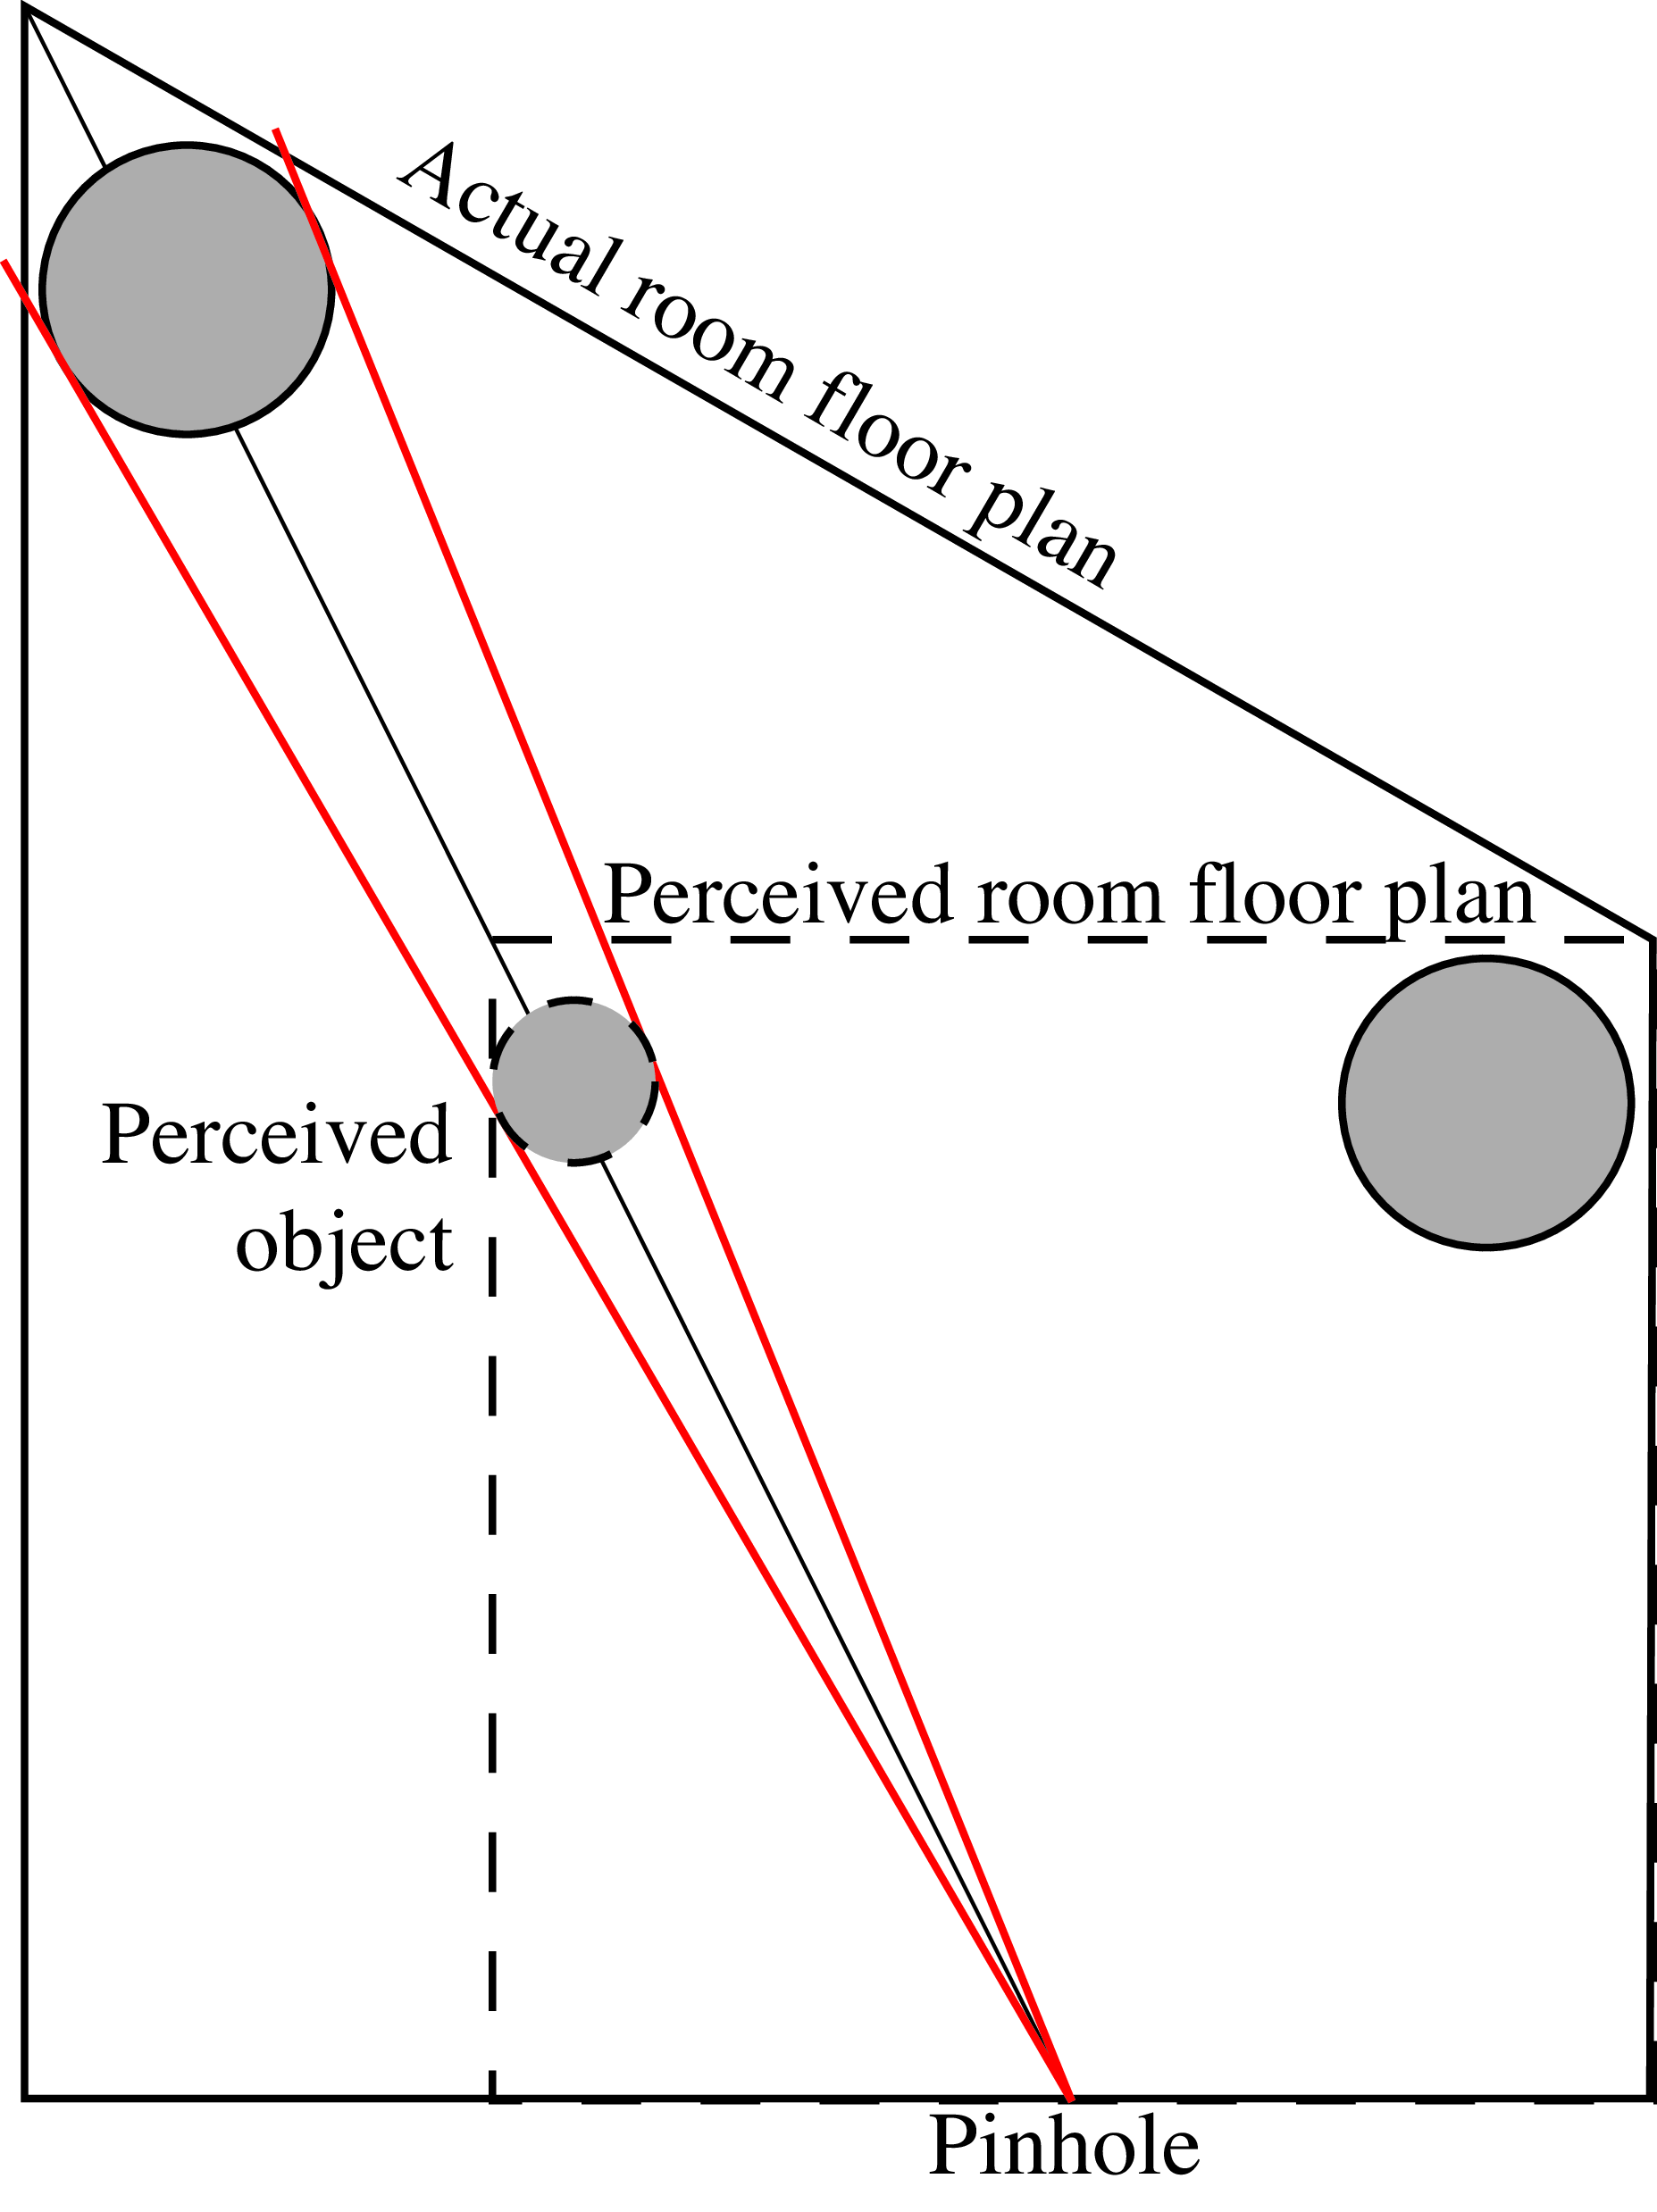
\includegraphics[width=0.3\textwidth, angle=90]{imagenes/chapter1/AmesRoom}}\\
        \subfloat{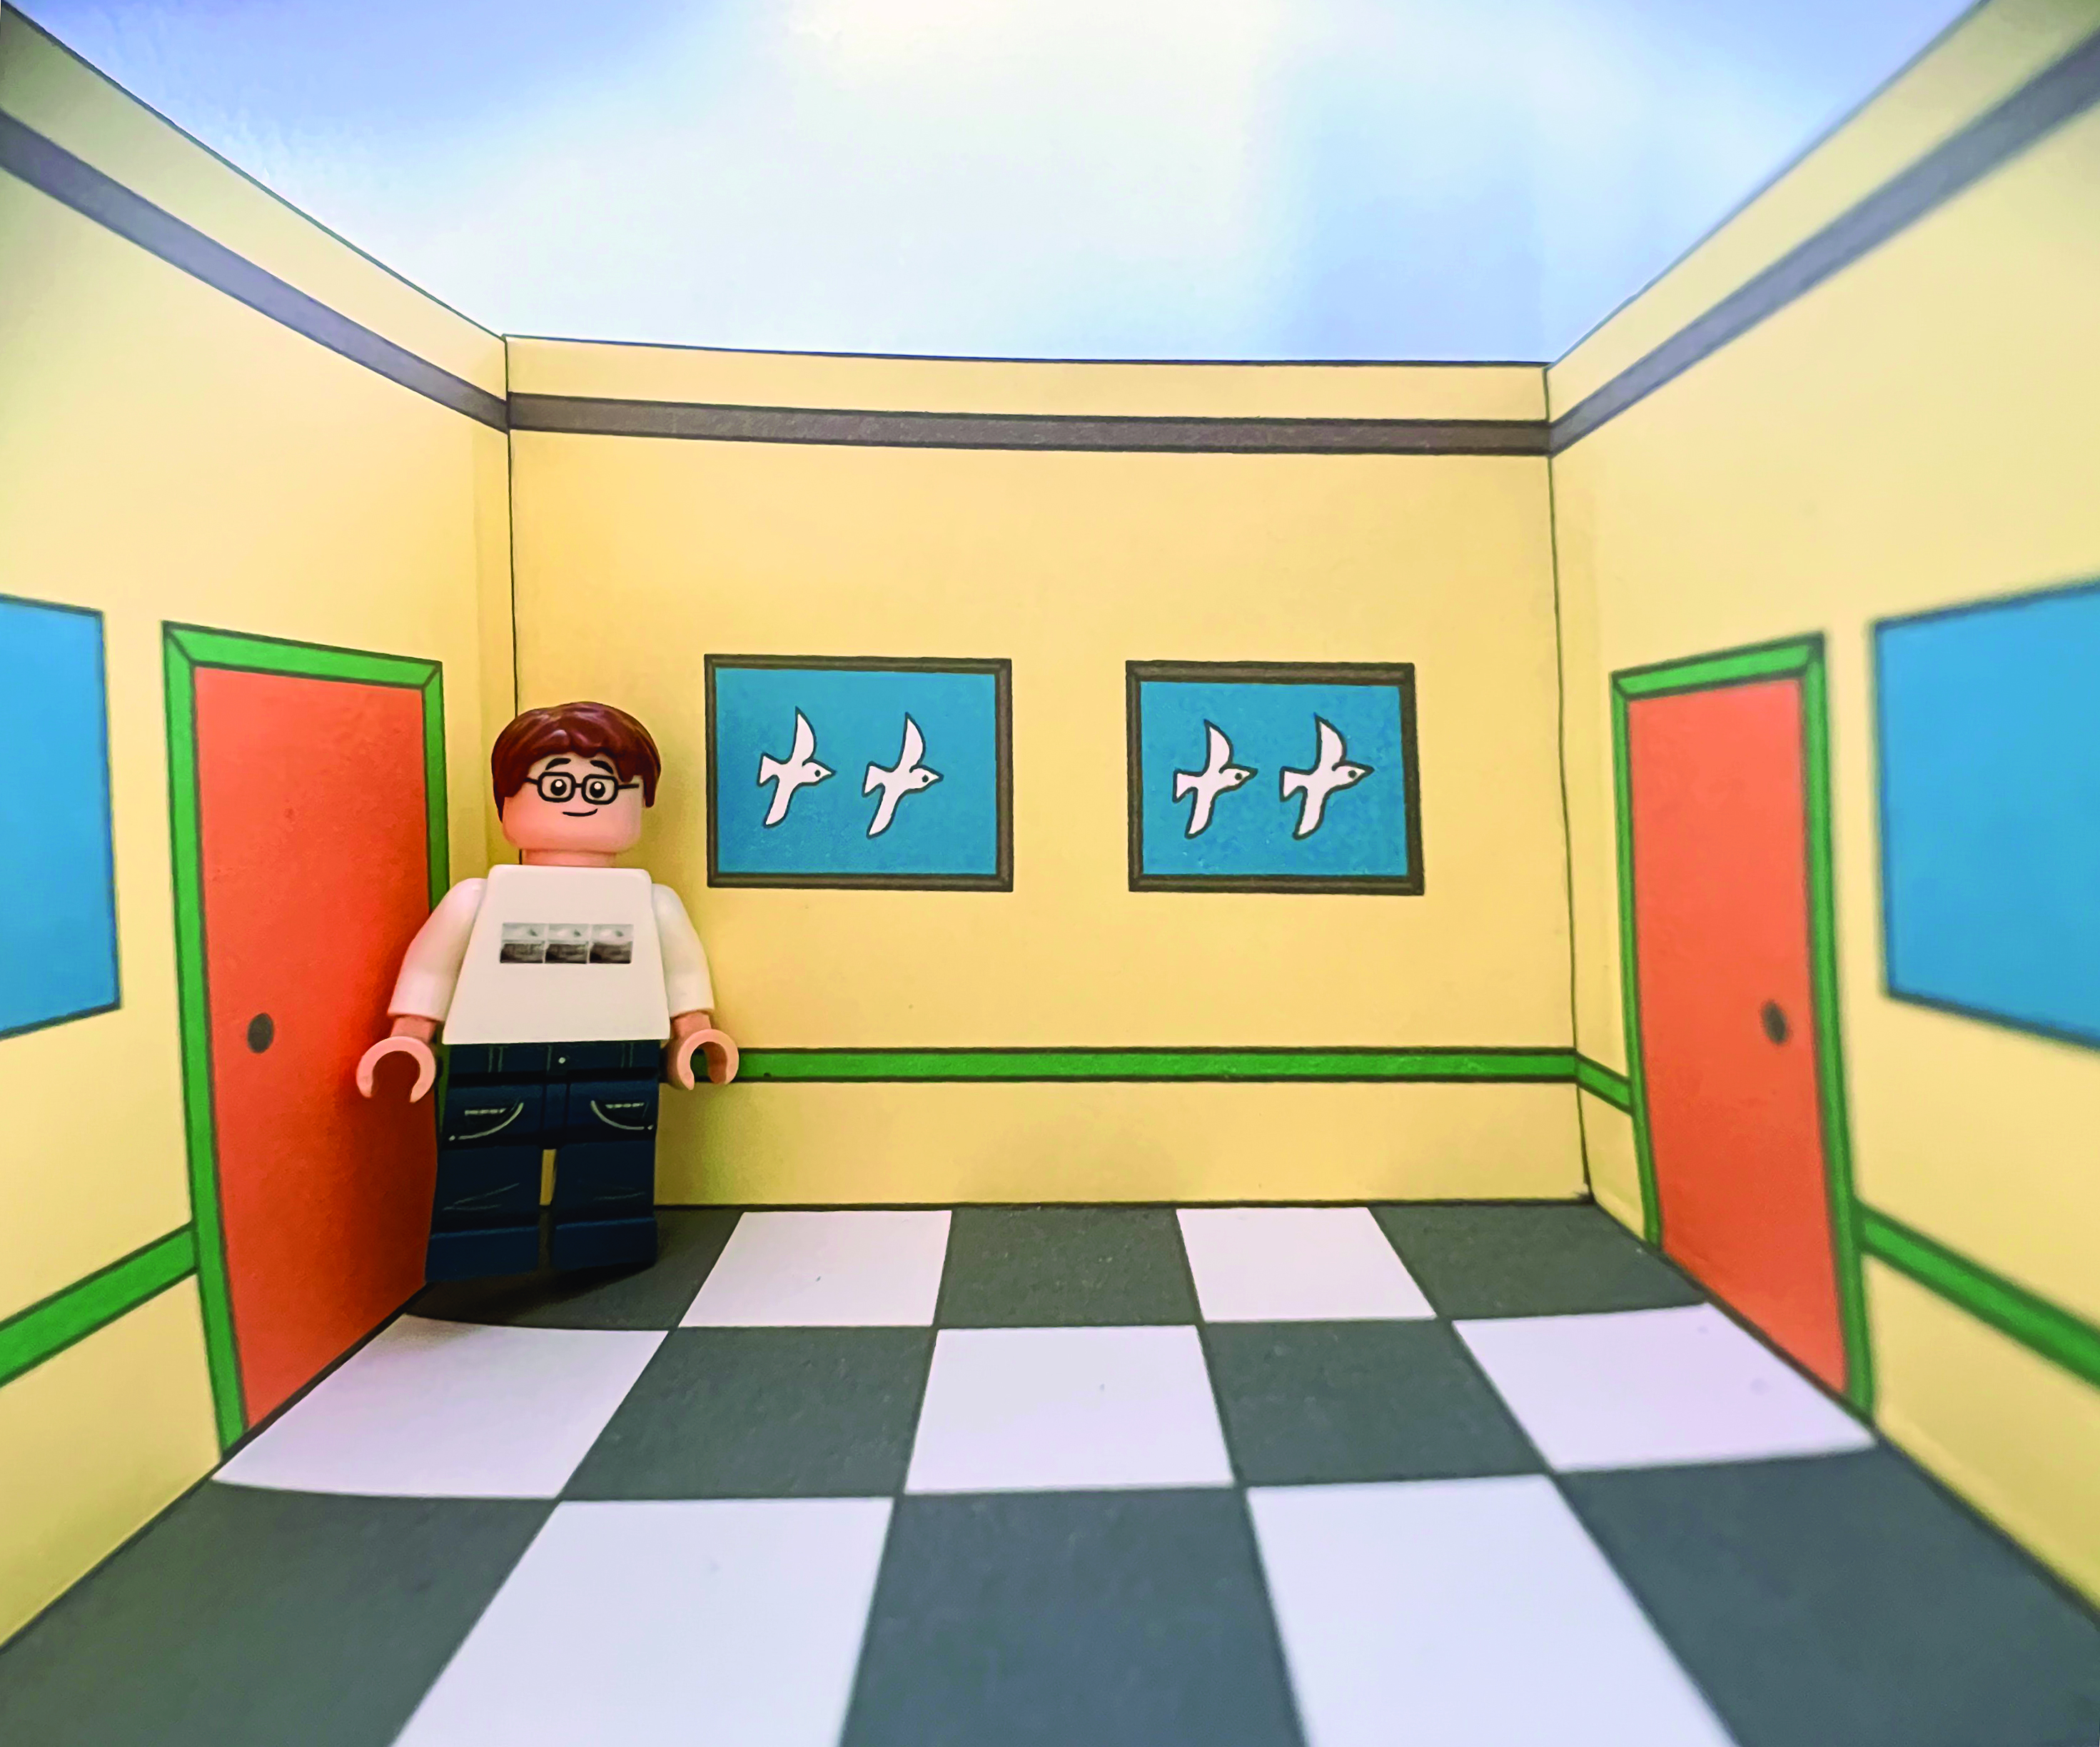
\includegraphics[width=0.5\textwidth]{imagenes/chapter1/LegoLeftSmall}}
        \subfloat{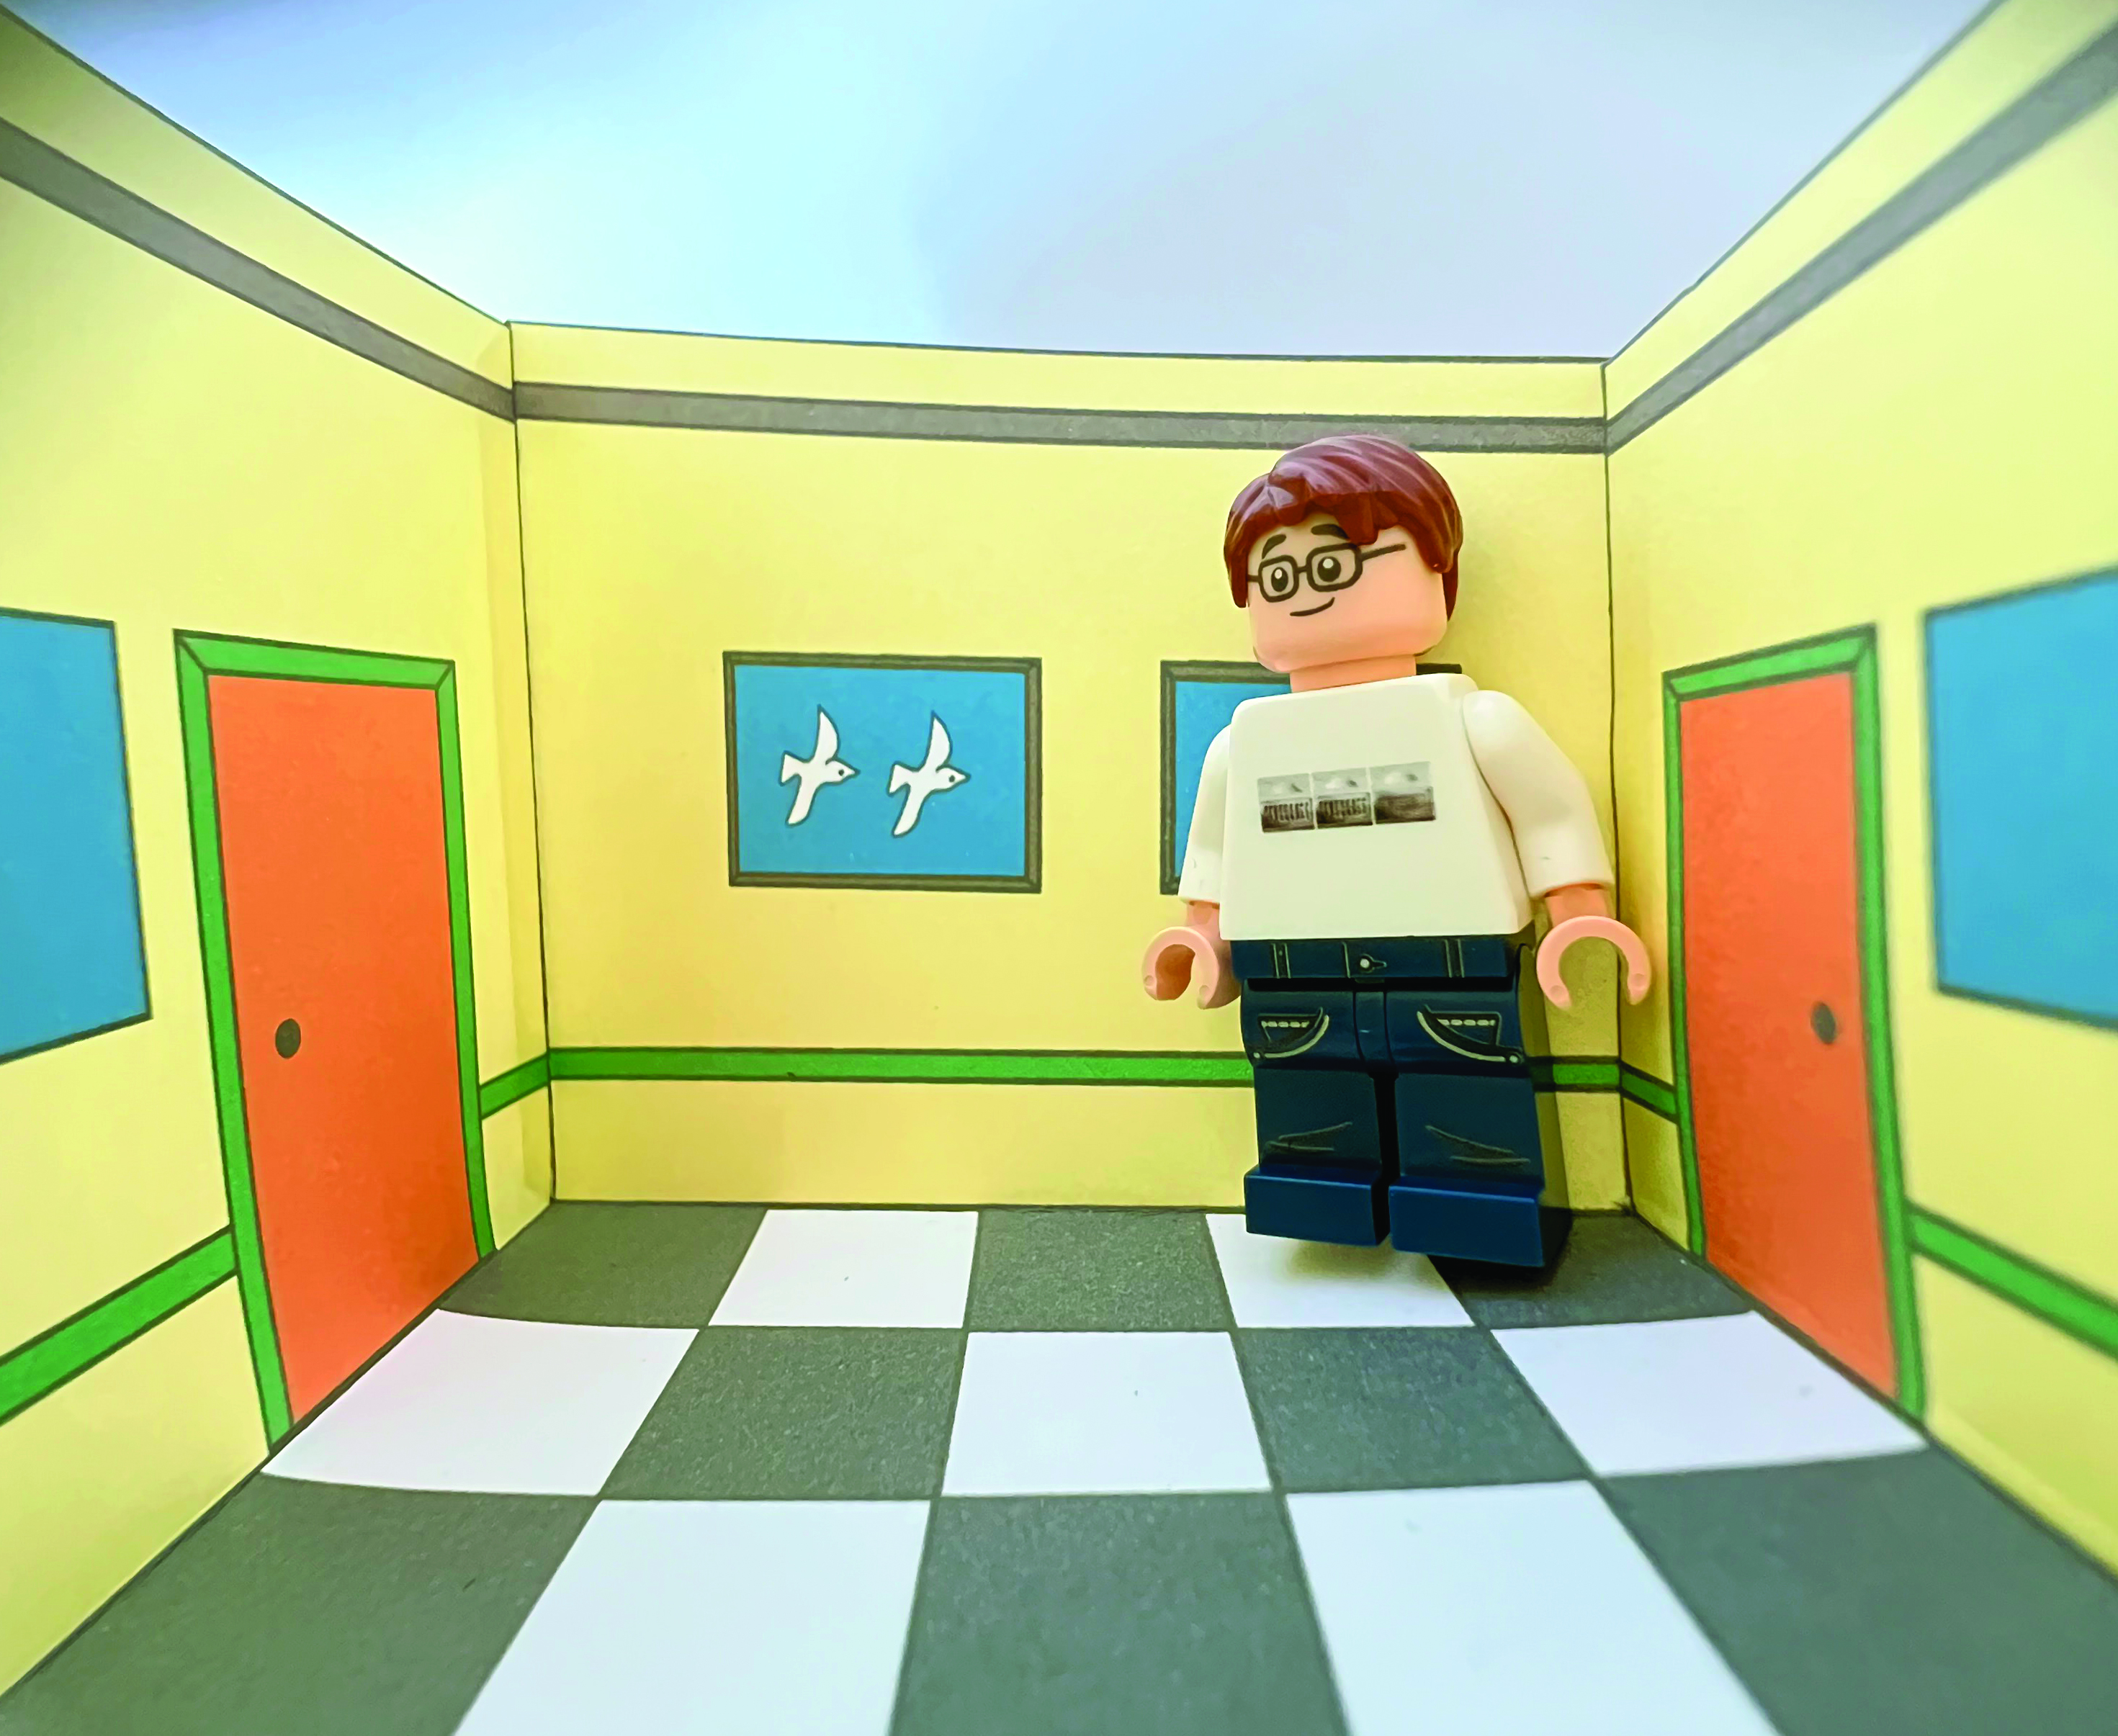
\includegraphics[width=0.505\textwidth]{imagenes/chapter1/LegoRightBig}}
    \end{center}
    \caption{Ilusión óptica, un mismo objeto se percibe de tamaño diferente\footnotemark.}
    \end{figure}
    \end{columns}
    \addtocounter{footnote}{-1}
    \footcitetext{CriminisiApplications}
    \stepcounter{footnote}
    \footcitetext{VisionBookMIT}
\end{frame}

\note{
  Es especialmente útil en situaciones donde no es práctico capturar múltiples imágenes desde diferentes ángulos.
  Sin embargo la aplicación de mediciones monoculares en entornos no controlados plantea diversas dificultades.
  Como se observa en la Figura, es muy fácil provocar ilusiones ópticas de profundidad y tamaño, haciendo esta tarea realmente compleja.
  No obstante, el interés en el campo ha crecido en paralelo con los grandes avances en visión por computador y aprendizaje profundo.
  El objetivo de este trabajo es automatizar y facilitar dicho procedimiento.
  Ya que, en el caso de los métodos clásicos la metrología se hace mediante labores manuales extensas de calibración de la escena.
}

\begin{frame}
  \frametitle{Aplicaciones}
  \begin{columns}
    \column{0.5\textwidth}
    \begin{itemize}
      \item \textbf{Entornos forenses}\footnotemark: Estimación de la altura de sospechosos a partir de grabaciones.
      \item \textbf{Biomecánica}\footnotemark[\value{footnote}]: Análisis del movimiento.
      \item \textbf{Reconstrucción de escenas}\footnotemark[\value{footnote}].
      \item \textbf{Geometría en pinturas}\footnotemark[\value{footnote}].
    \end{itemize}
    \column{0.5\textwidth}
    \begin{figure}[!ht]
      \begin{center}
        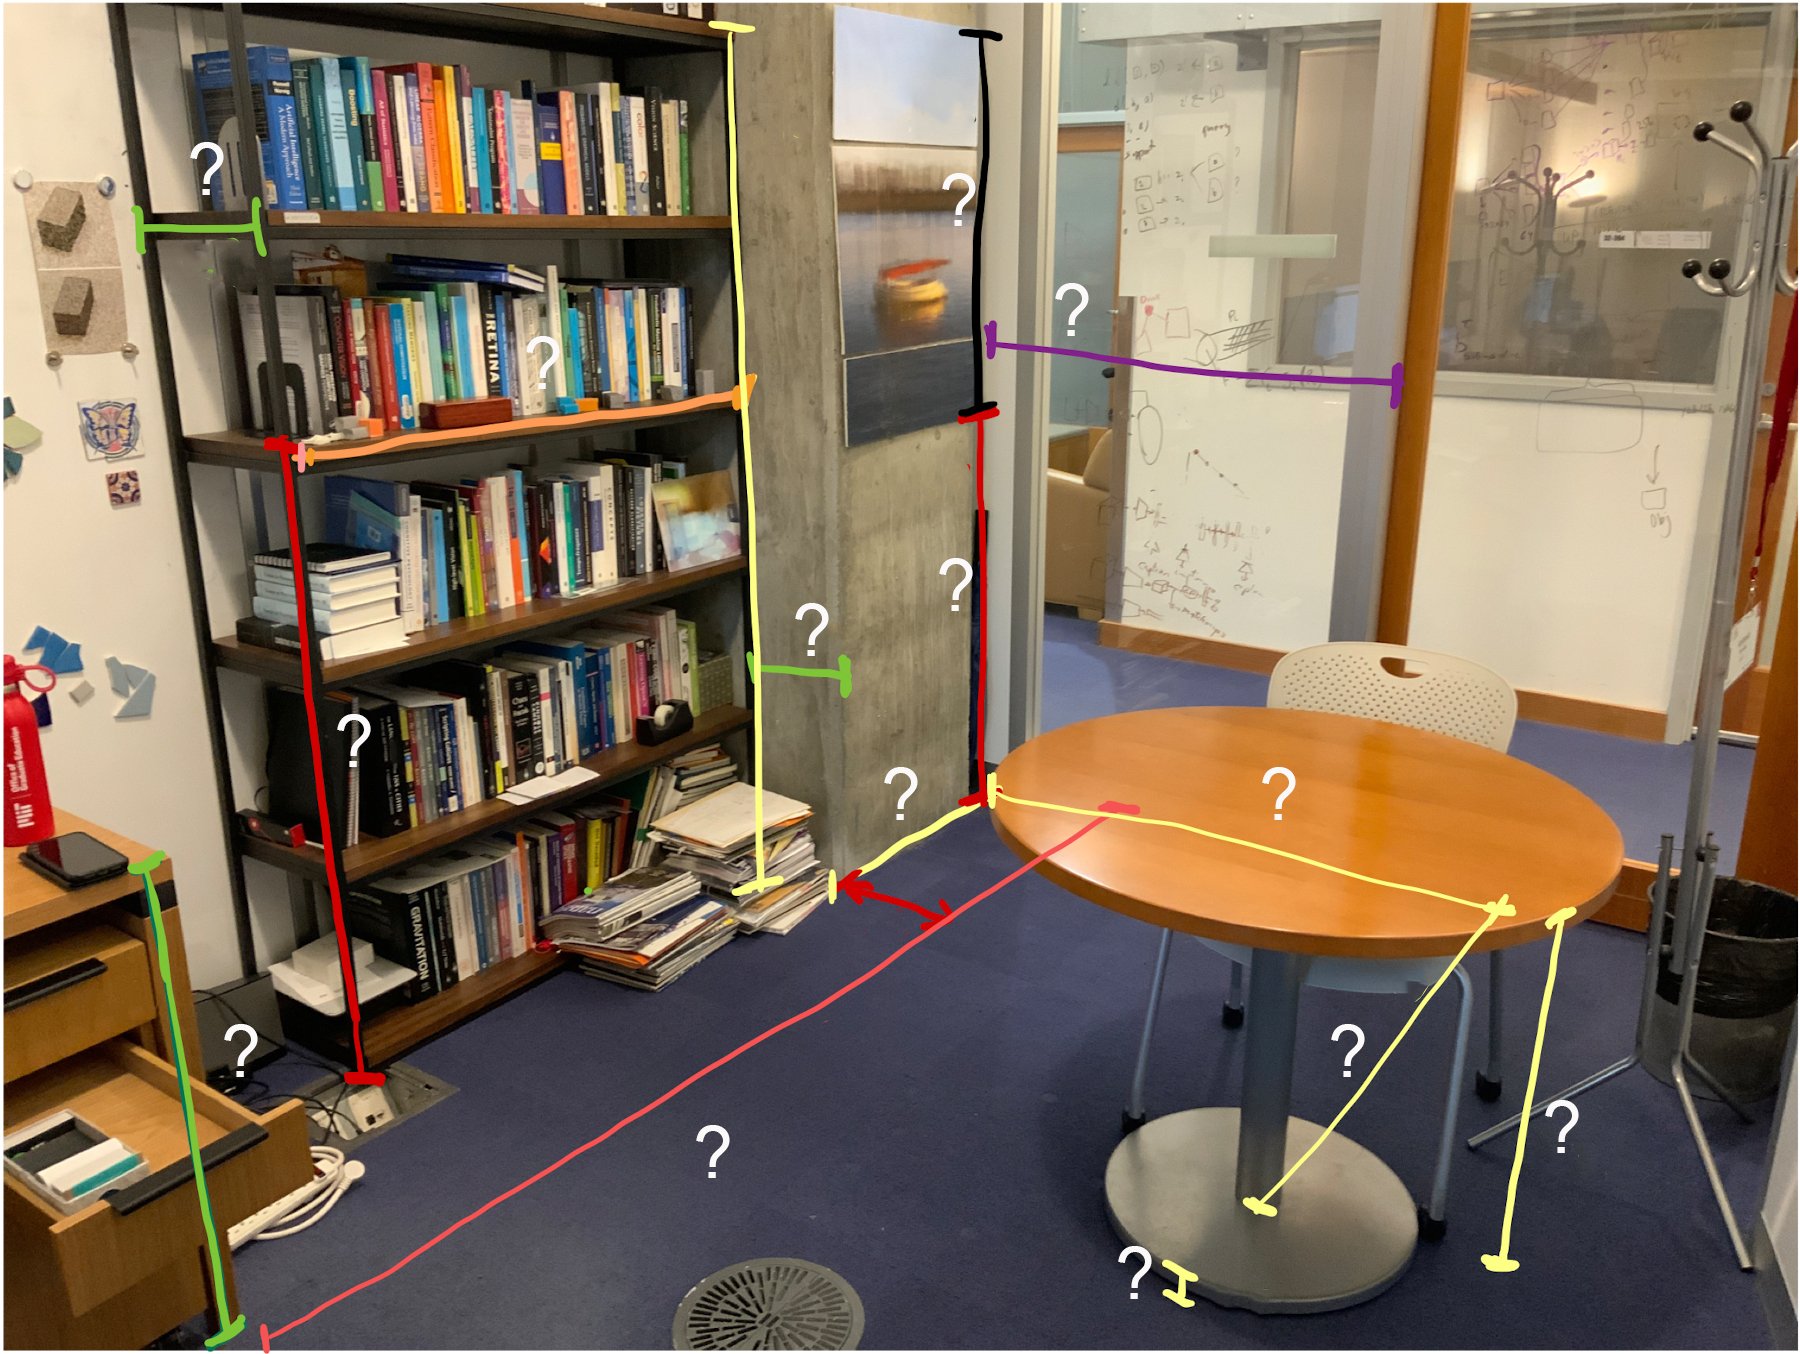
\includegraphics[width=0.80\textwidth]{imagenes/chapter1/office-measurements.jpg}
      \end{center}
      \caption{Ejemplo visual de información extraíble a partir de una sola imagen\footnotemark.}
    \end{figure}
  \end{columns}
  \addtocounter{footnote}{-1}
  \footcitetext{CriminisiApplications}
  \stepcounter{footnote}
  \footcitetext{VisionBookMIT}
\end{frame}

\note{
  Contribuir al desarrollo de soluciones para extraer medidas de una sola imagen puede tener un impacto significativo
  en diversos ámbitos. Desde entornos forenses y la biomecánica, hasta la reconstrucción y análisis de geometrías de las escenas.
  Fíjense, por ejemplo, en la Figura a la derecha que ilustra un ejemplo de un análisis de escena realizable por metrología monocular.
}

\subsection{Objetivos}
\begin{frame}
  \frametitle{Objetivos}
  \begin{figure}[!ht]
    \begin{center}
      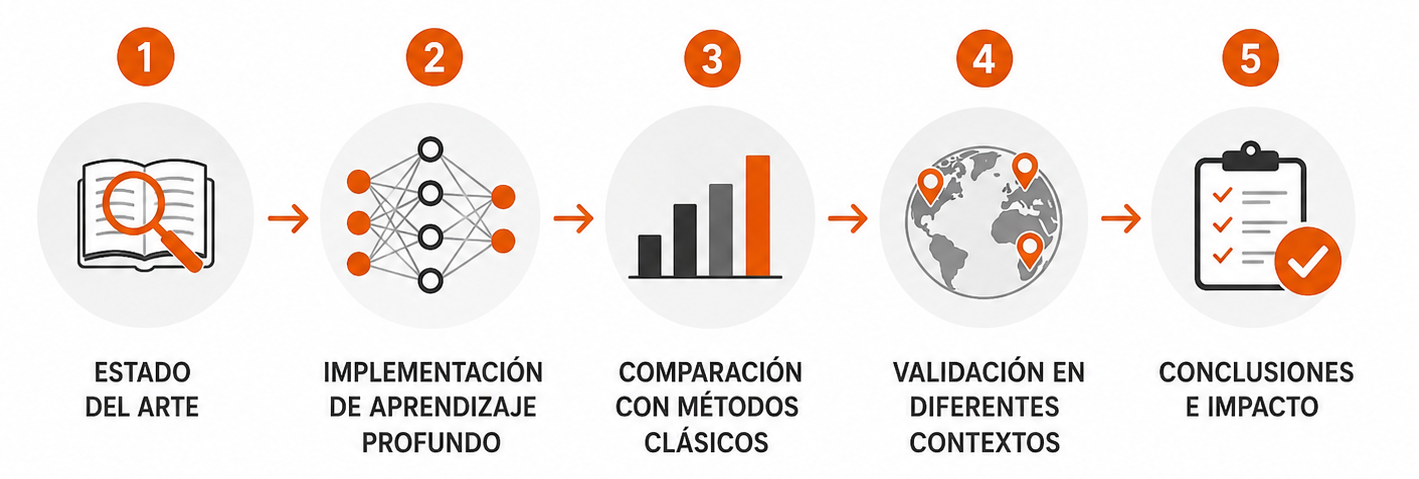
\includegraphics[width=0.95\textwidth]{imagenes/chapter1/test-crop.png}
    \end{center}
    \caption{Objetivos del proyecto\footnotemark.}
  \end{figure}
  \footnotetext{Ilustración generada por inteligencia artificial (IA).}
\end{frame}

\note{
  Por lo tanto, estos serán los objetivos de este proyecto.
  Realizar un estudio del estado del arte. Obtener una implementación que permita automatizar el proceso para cualquier cámara y escena.
  Realizar una comparativa frente a los métodos clásicos y obtener conclusiones y posibles líneas de investigación.
}
